\chapter[第五章]{} % (fold)
\label{cha:chapter5}

\section*{数值积分}

\subsection{问题}

\begin{equation}
    I = \int_0^1 \frac{\mathrm{arctan}x}{x^{\frac{3}{2}}} \mathrm{d}x
\end{equation}



\begin{enumerate}[(1)]
    \item 用 Romberg 公式计算改积分,使误差不超过 $\frac{1}{2}\times 10^{-7}$;
    \item ⽤复化 3 点 Gauss-Legendre 公式计算它,使误差不超过 $\frac{1}{2}\times 10^{-7}$。
\end{enumerate}

\subsection{分析}

\subsubsection{复化 Romberg 公式的分析}

\begin{enumerate}[(1)]
    \item 首先用递推关系求梯形公式:
    \begin{align}
        T_1 &= h(\frac{1}{2}f(a)+\frac{1}{2}f(b)) \\
        T_{2n} &= \frac{1}{2}T_n + \frac{h(n)}{2}\sum\nolimits_{n=0}^{n-1}f(x_{k+1/2})
    \end{align}

    \item 利用梯形公式求 Simpson 公式:
    \begin{equation}
        S_n(f) = \frac{4}{3}T_{2n}(f) - \frac{1}{3}T_n(f)
    \end{equation}

    \item 利用 Simpson 公式求 Cotes 公式:
    \begin{equation}
        C_n(f) = \frac{16}{15}S_{2n}(f)-\frac{1}{15}S_n(f)
    \end{equation}

    \item 最后用 Cotes 求 Romberg 公式:
    \begin{equation}
        R_n(f) = \frac{64}{63}C_{2n}(f)-\frac{1}{63}C_n(f)
    \end{equation}
\end{enumerate}

\subsubsection{Gauss-Legendre 求积公式分析}

\begin{enumerate}[(1)]
    \item $[-1,1]$ 上的3点Gauss-Legendre公式:
    \begin{equation}
        \int_{-1}^1 g(x)\mathrm{d}x \approx \frac{5}{9}g(-\sqrt{\frac{3}{5}}) + \frac{8}{9}g(0) + \frac{5}{9}g(\sqrt{\frac{3}{5}})
    \end{equation}

    \item 一般区间 $[a,b]$ 上的 Gauss 公式:
    
    令 $x_k = \frac{a+b}{2}+\frac{b-a}{2}t_k$,$A_k = \frac{b-a}{2}\tilde{A}_k$,$k=0:n$

    \item 由于 Gauss 求积公式的节点不具有递推性,因此考虑用截断误差计算节点的数量, Gauss-Lengdre 公式的截断误差为:
    \begin{multline}
        R(f) = \int _a^b f(x)\mathrm{d}x - \sum\nolimits_{k=0}^n A_kf(x_k) = \frac{f^{2n+2}(\xi)}{(2n+2)!} \int_a^b W_{n+1}^2(x)\mathrm{d}x, \\
        W_{n+1}(x) = \prod\nolimits_{j=0}^n (x-x_j), \quad \xi \in (a,b)
    \end{multline}

    由于导数计算不太方便,并且还需要求函数的最大值,增加了程序的复杂性。考虑到使用分段积分可以极大地减少计算量(后面结论分析会给出一个分段与不分段计算时间的对比),因此用每次将区间长度减小一半,计算出一个 $R_n(f)$,用前后两次结果的差值作为误差判断的依据(后验误差),只要误差小于误差限,就停止计算。

\end{enumerate}

\subsubsection{待积函数分析}

待求积分的函数为:

\begin{equation}
    g(x) = \frac{\mathrm{arctan}x}{x^{3/2}}
\end{equation}

该函数的图像如图\ref{fig:f}所示,是一个奇异函数,在 $x=0$ 处有奇异点,值为 $+\infty$,用 Romberg 公式求积时需要用到 $x=0$ 处的值。在 $[0,x_0]$ 上的积分用右矩形公式的两倍近似,即 $\int_0^{x_0} g(x) \mathrm{d}x \approx 2\cdot x_0 \cdot g(x_0) $,保证近似值小于一半的误差限,即 $2\cdot x_0 \cdot g(x_0) \leq 1/2 \times 1/2 \times 10^{-7}$;

为了减少计算量,在 $[x_0, 1]$ 上,做分段积分,分别对 $[x_0,1\times 10^{-9}]$、$[1\times 10^{-9},1\times 10^{-4}]$、$[1\times 10^{-4},1]$做Romberg积分,每一段的误差都要求小于 $1/6 \times 1/2 \times 10^{-7}$,这样保证总的误差不超过 $ 1/2 \times 10^{-7}$。

\begin{figure}[ht]
    \centering
      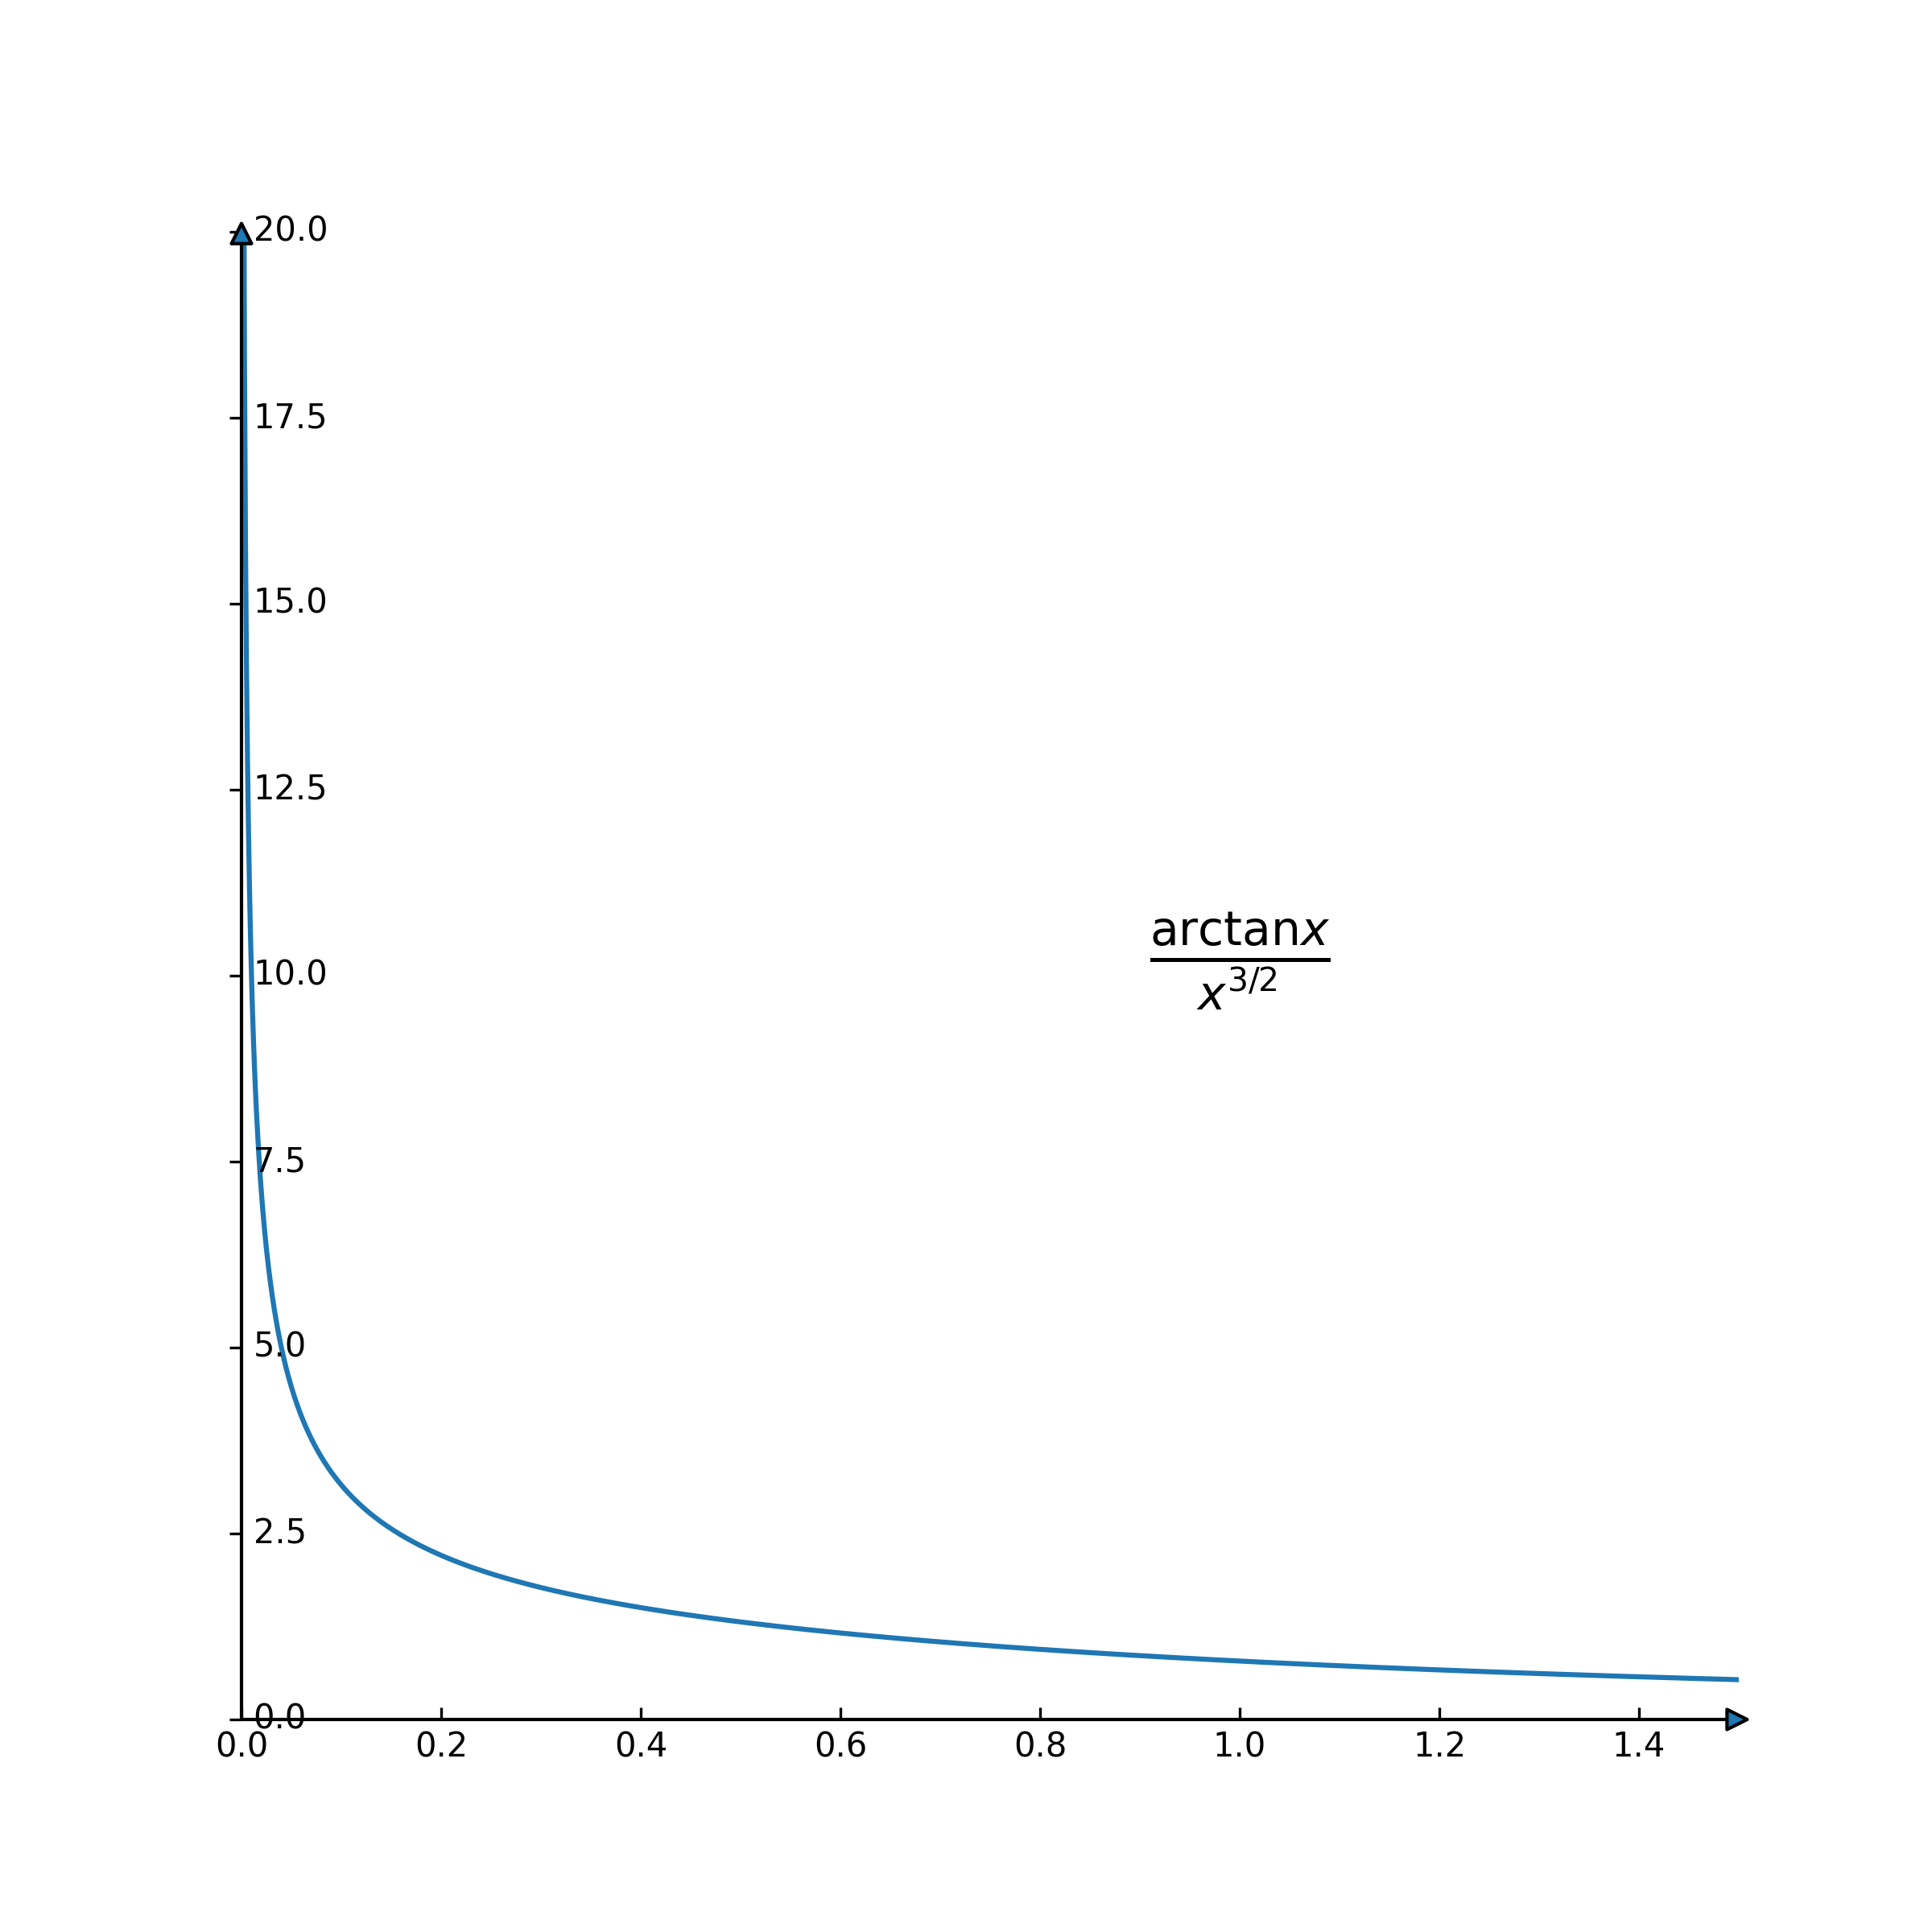
\includegraphics[width=0.5\textwidth]{fq3}
      \caption{$(\mathrm{arctan}x)/(x^{3/2})$ 图像}
      \label{fig:f}
\end{figure}

\subsection{程序}

\subsubsection{q3\_romberg.py}

\begin{lstlisting}[style = python]
    import math
    import time
    import os, sys
    
    RESULT_FILE = os.path.join(os.path.dirname(os.path.abspath(__file__)), 'q3_romberg_result.txt')
    
    def print_row(lst, n):
        print('n =: ', n, ', ',' '.join('%11.8f, ' % x for x in lst))
        with open(RESULT_FILE, "a+") as fo:
            fo.write('n: {0}, '.format(n))
            for x in lst:
                fo.write('{0}, '.format(x))
            fo.write('\n')
    
    
    def romberg(f, a, b, eps=1e-8):
        """Approximate the definite integral of f from a to b by Romberg's method.
        eps is the desired accuracy."""
        R = [[0.5 * (b - a) * (f(a) + f(b))]]  # R[0][0]
        print_row(R[0], 1)
        n = 1
        while True:
            h = float(b - a) / 2 ** n
            R_row_tmp = []
            R_row_tmp_0 = 0.5*R[n-1][0] + h*sum(f(a+(2*k-1)*h) for k in range(1, 2**(n-1)+1))
            R_row_tmp.append(R_row_tmp_0)
            for m in range(1, min(n, 3)+1):
                tmp = R_row_tmp[m-1] + (R_row_tmp[m-1] - R[n-1][m-1]) / (4 ** m - 1)
                R_row_tmp.append(tmp)
            R.append(R_row_tmp)
            print_row(R[n], 2**n)
            if n >= 4 and abs(R[n-1][3] - R[n][3])/255.0 < eps:
                return R[n][-1]
            n += 1
    
    '''
    description: 处理反常积分奇异点为 0 的情况,返回
    return {*} 
    '''
    def Improper_deal(f, a, b, err=1e-8):
        m = 2
        x = a + (b-a)/m
        while 2.0*f(x)*x > err:
            m = m * 2.0
            x = a + (b-a)/m
        return x
    
    def expression0(x):
        return 1.0/x
    
    def expression1(x):
        return math.atan(x)/(pow(x, 1.5))
    
    def main():
        a = Improper_deal(expression1, 0, 1, (0.5e-7)/2.0)
        print(a)
        with open(RESULT_FILE, "a+") as fo:
            fo.write('a = {0}, '.format(a))
            fo.write('\n')
        print('int3')
        int3 = romberg(expression1, 1e-4, 1, (0.5e-7)/6.0) # 
        print('int2')
        int2 = romberg(expression1, 1e-9, 1e-4, (0.5e-7)/6.0) #
        print('int1')
        int1 = romberg(expression1, a, 1e-9, (0.5e-7)/100.0) # 100.0
        int_all = int1+int2+int3
        print('result is {0} .'.format(int_all))
        with open(RESULT_FILE, "a+") as fo:
            fo.write('n: {0}, '.format(int_all))
            fo.write('\n')
    
    
    if __name__ == "__main__":
        time_start = time.time()
        if os.path.exists(RESULT_FILE):
            os.remove(RESULT_FILE)
        main()
        time_end=time.time()
        print('time cost {0} s. '.format(time_end - time_start))
        with open(RESULT_FILE, "a+") as fo:
            fo.write('time cost {0} s. \n'.format(time_end - time_start))
\end{lstlisting}

\subsubsection{q3\_gauss\_legendre.py}

\begin{lstlisting}[style = python]
    import time
    import math
    import os, sys
    
    RESULT_FILE = os.path.join(os.path.dirname(os.path.abspath(__file__)), 'q3_gauss_legendre_result.txt')
    
    def Gauss_Legendre(f, a, b):
        Int = (b-a) * (5.0 * f(0.5*(a+b-(b-a)*pow(3.0/5.0, 0.5))) + \
            8.0 * f(0.5*(a+b)) + 5.0 * f(0.5*(a+b+(b-a)*(pow(3.0/5.0, 0.5))))) / (9.0*2.0)
        return Int
    
    def Com_Gauss_Legendre(f, a, b, n):
        h = (b-a)/n
        Int_Sum = 0.0
        for i in range(1, n+1):
            x0 = a + (i - 1.0) * h
            x1 = a + i * h
            Int_Sum += Gauss_Legendre(f, x0, x1)
        return Int_Sum
    
    def Get_Com_Gauss_Legendre(f, a, b, err):
        Int_Last = 0
        i = 0
        while True:
            Int = Com_Gauss_Legendre(f, a, b, 2 ** i)
    
            print('n: {0}, {1}'.format(2**i, Int))
            with open(RESULT_FILE, "a+") as fo:
                fo.write('n: {0}, {1} \n'.format(2**i, Int))
    
            if abs(Int - Int_Last) <= err:
                return Int, i
            else:
                Int_Last = Int
                i += 1
    
    def expression1(x):
        return math.atan(x)/(pow(x, 1.5))
    
    def main():
        print('int3')
        int3, n3 = Get_Com_Gauss_Legendre(expression1, 1e-5, 1, (0.5e-7)/6.0) # 
        print('int2')
        int2, n2 = Get_Com_Gauss_Legendre(expression1, 1e-10, 1e-5, (0.5e-7)/6.0) #
        print('int1')
        int1, n1 = Get_Com_Gauss_Legendre(expression1, 0, 1e-10, (0.5e-7)/6.0) # 100.0
        int_all = int1+int2+int3
        n_times = 2**(n1+n2+n3)
        print('result is {0} , n is {1}'.format(int_all, n_times))
        with open(RESULT_FILE, "a+") as fo:
            fo.write('result is {0} , n is {1}'.format(int_all, n_times))
            fo.write('\n')
    
    if __name__ == "__main__":
        time_start = time.time()
        if os.path.exists(RESULT_FILE):
            os.remove(RESULT_FILE)
        main()
        time_end=time.time()
        print('time cost {0} s. '.format(time_end - time_start))
        with open(RESULT_FILE, "a+") as fo:
            fo.write('time cost {0} s. \n'.format(time_end - time_start))
\end{lstlisting}

\subsection{算例}

\begin{equation}
    I = \int_0^1 \frac{\mathrm{arctan}x}{x^{\frac{3}{2}}} \mathrm{d}x
\end{equation}

分段的考虑是分3段,调整3段的长度,尽量使每一段上面的计算次数相等,这样应该可以使总的计算次数最少。

用 Romberg 求积公式的实际积分区间是$[1.110223025\times 10^{-16},1\times 10^{-9}]$、$[1\times 10^{-9},1\times 10^{-4}]$、$[1\times 10^{-4},1]$,计算出来的结果是:$1.897097415$;

用 Gauss-Legendre 求积公式实际积分区间是$[0,1\times 10^{-10}]$、$[1\times 10^{-10},1\times 10^{-5}]$、$[1\times 10^{-5},1]$,计算出来的结果是:$1.897095603$。

\subsection{结论}

算术解的结果为(使用\href{https://www.wolframalpha.com/}{wolframalpha.com}计算):
\begin{multline}
    y = -\frac{log(x - \sqrt{2x} + 1)}{\sqrt{2}} + \frac{log(x + \sqrt{2x} + 1)}{\sqrt{2}} {} \\
    - \sqrt{2} tan^{-1}(1 - \sqrt{2x}) + \sqrt{2} tan^{-1}(\sqrt{2x} + 1) - \frac{2 tan^{-1}(x)}{\sqrt{x}}
\end{multline}

因此准确解是:$1.897095623$。

\subsubsection{复化 Romberg 公式}

对比准确解可以看到,实际误差为$1.8\times 10^{-6}$,大于所要求的的 $\frac{1}{2}\times 10^{-7}$,且计算值略大于真实值,分析后应该是在 $[x_0,1\times 10^{-9}]$ 这段上误差太大,因为在 $x_0$ 处的值还是太大了,因此将这段的误差设为 $1/2\times 10^{-9}$,其他两段的误差设定保持 $1/6 \times 1/2 \times 10^{-7}$,再次计算出来的结果是 $1.897095976$,误差是 $3.5\times 10^{-7}$,达到了误差的要求。

在没有分段积分时,程序跑了一周多也没有收敛到误差要求内,在设定好合适的分段积分区间后,程序只运行了 0.2 s 就收敛到误差要求内,效率提升很大。

\subsubsection{Gauss-Legendre 求积公式}

对比准确解可以看到,使用分段后的 Gauss-Legendre 求积公式计算结果的误差为 $2.0\time 10^{-8}$,达到了误差的要求。

与Romberg求积类似,在没有分段积分时,程序跑了一周多也没有收敛到误差要求内,在设定好合适的分段积分区间后,程序只运行了 1.9 s 就收敛到误差要求内,效率提升很大。

\subsubsection{总结}

计算奇异函数,分段计算很有必要,可以极大地减少计算量,提高计算速度。


% chapter chapter5 (end)